\documentclass[10pt]{book}
\usepackage{graphicx}
\usepackage{exercise}
\usepackage{url}
\usepackage[width=5.5in,height=8.0in,
  hmarginratio=3:2,vmarginratio=1:1]{geometry}


\begin{document}
\chapter {Directed Graphs}
\section{Question}
\subsection{Why do directed graphs matter?}
Imagine that it’s 2am during finals week, and you’re scrambling to finish your research paper on topica obscura. Your adrenaline jumps when you finally find a relevant Wikipedia article, with links to more Wikipedia articles! You start clicking away, jumping from page to page in search of facts. An hour later, you realize you’re still clicking, but these are pages you’ve already visited. No matter which link you click, you can’t seem to discover any new pages! 

If this situation has ever happened to you, then you’ve unknowingly (and unfortunately) stumbled upon a knot in Wikipedia. Knots are a unique property of directed graphs. To understand them, it’s necessary to have a basic understanding of directed graphs.
\section{Methodology}
\subsection{Directed graph implementation}
	 	 	
So far in this book, all of the graphs we’ve encountered have been undirected graphs. In an undirected graph, a single edge connects two vertices, and an edge from vertex V to vertex W is the same as an edge from W to V. This abstraction works well to describe some real-world systems (such as social networks and transportation networks), but it isn’t detailed enough to describe the Internet, including Wikipedia. 

On Wikipedia, connections between pages do not have to be mutual. Page A might link readers to page B, but page B doesn’t have to include any links to page A. Is there an edge between A and B? Absolutely, but knowing that an edge exists is not enough information. To understand the relationship between pages A and B, we need two bits of information: whether A links to B, and whether B links to A . This is the essence of a directed graph.

\begin{figure}[here]
 \centering
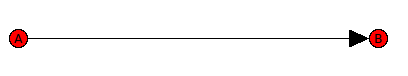
\includegraphics[scale=0.6]{../Images/DirectedGraphExample.png}
\end{figure}
In a directed graph, edges are replaced by arcs. Wikipedia explains that “an arc e = (x,y) is considered to be directed from x to y”. Arcs are sometimes called directed edges as well. 

As mentioned before, knots are a unique (and sometimes cruel) property of directed graphs. Wikipedia explains that “a knot in a directed graph is a collection of vertices and edges with the property that every vertex in the knot has outgoing edges, and all outgoing edges from vertices in the knot terminate at other vertices in the knot. Thus it is impossible to leave the knot while following the directions of the edges.” In other words, if you start on any vertex in a knot

we mentioned the idea of knots in Wikipedia. We wondered whether such a thing was even possible? Given that there’s 3,811,000+ articles on Wikipedia, it seemed unlikely that there would be a knot with no outlinks, but we decided to investigate.

Before we wrote an algorithm to find a knot in a directed graph, we wanted to extend Graph.py to support directed graphs. So we wrote DirectedGraph.py, which you can download at https://raw.github.com/nrubin/RachelAndNoamsDirectedGraphs/master/DirectedGraph.py. We recommend reading through DirectedGraph.py and making yourself familiar with the terminology. Note that Edges in DirectedGraph are represented by Arcs.

When we were designing DirectedGraph, we wanted to preserve the order of growth of Vertex and Arc lookups as they were in Graph. Therefore, we decided to keep track of out-arcs in the internal dictionary (inherited from \_\_DictWrapper\_\_), and in-arcs in an extra dictionary, called reverse\_graph. This way, we could keep the lookup of vertices and arcs fast while being able to address out-arcs and in-arcs separately. Having two dictionaries takes more memory, but not an order of magnitude more. Thus, the increase in memory complexity is negligible.

\subsection{Knots algorithm}

Now, back to knots. Our research has concluded that the only published knot algorithms are distributed algorithms. (see http://www.cs.utexas.edu/users/misra/scannedPdf.dir/KnotDetection.pdf) Distributed algorithms are designed to occur concurrently on multiple processors. Identical but distinct chunks of the algorithm run on each processor, and report to each other the results of their computation. These kinds of algorithms are ideal for large research projects, but we wanted an algorithm that would run on a single computer. To this end, we devised our own algorithm!

The main functionality of our algorithm is a modified version of breadth-first-search. Instead of searching for a specific value, it searches for all the vertices that can be reached from a specific starting vertex.  

\begin{verbatim}
  def _bfsknots(self, s):
        """
        Modified breadth-first search. Used to find knots.Returns the 
        set of vertices that are accessible by some path from s.

        s: start vertex
        """

        # initialize the queue with the start vertex
        queue = [s]
        visited = set()
        on_first_vertex = True
        while queue:

            # get the next vertex
            v = queue.pop(0)

            # skip it if it's already marked
            if v in visited: continue

            # if we're on the first vertex, we're not actually visting
            if v != s or not on_first_vertex: visited.add(v)
            on_first_vertex = False
            
            for x in self.out_vertices(v):
                #if its out vertices have been cached, update visited
                if x in self._knot_cache.keys():
                    visited.update(self._knot_cache[x])
                    visited.add(x)
                    
                #otherwise add it to the queue
                elif x not in self._knot_cache.keys():
                    queue.append(x)

        return visited
\end{verbatim}

If the $S_v = S_x \; \forall \; x \; \epsilon \; S_v$, holds for a specific vertex, then a knot must exist at that vertex.

\begin{verbatim}
     def _knot_at_v(self, v):
        """
        Given a vertex v, finds whether each of its out vertices
        are all accessible from each other, and not accessible from
        any other vertex.
        
        Returns True if this is case; indicates v is entrance to knot.
        """
        t = self._knot_cache.get(v, None)

        if len(t) == 0:
            return False
            
        for w in self._knot_cache[v]:
                s = self._knot_cache.get(w, None)
                if len(s) == 0:
                    return False
                x = s.symmetric_difference(t)
                if x != set([]):
                    return False

        return True
\end{verbatim}

The function \verb“has_knot” ties the previous two conditions together, by returning True if a knot exists somewhere in the graph.
\begin{verbatim}
    def has_knot(self):
        """
        Returns true if directed graph has a knot.
        """
        self._knot_cache = {}
        #build the cache of which vertices are accessible from which
        for v in self:
            self._knot_cache[v] = self._bfsknots(v)

        #searches for knot
        for v in self:
            if self._knot_at_v(v):
                return True
        return False

\end{verbatim}

\begin{exercise}
 Determine the order of growth of has\_knots experimentally. Hints:
\begin{enumerate}
 \item Use DirectedGraph.add\_random\_edges to generate a few thousand graphs of different sizes.

\item For each graph, time how long it takes to check if it has a knot.

\item Plot the time it took to check if the graph has a knot vs. the number of vertices the graph has. Also plot against the number of edges the graph has.

\item What has more of an effect on the runtime has\_knots, vertices or edges?

\item From your figures, determine the order of growth of has\_knots.
\end{enumerate}

\end{exercise}

\begin{exercise}
 Find all the knots in a directed graph.
\begin{enumerate}
 \item Write a function (or modify an existing one) to return a list of all knots in a graph.
\item Using your answer from the previous question, write a function that returns a list of all the vertices that serve as entry points into knots.
\end{enumerate}

\end{exercise}
\subsection{Parsing Wikipedia}

To find knots in Wikipedia, we selected 558 distinct subsets of Wikipedia articles, organized by index. For example, articles about Neurbiology was a subset, as were articles about Zimbabwe. In all, these subsets contained about 321,000 articles, or 10\% of Wikipedia. We chose to examine subsets because Wikipedia as a whole was too large for us to process\footnote{If you’re interested in the whole graph of Wikipedia, we recommend checking out research done by Stephen Dolan at Trinity College Dublin. His research is online here: \url{http://mu.netsoc.ie/wiki/}}. 

\section{Results}
\subsection{Knots in Wikipedia}
Of the 558 subgraphs we examined, 38\% contained at least one knot. This indicates that if you are reading similar articles, there is a chance you will get stuck in a knot and see the same articles repeatedly. However, this does not mean the Wikipedia as a whole has a knot, since we only looked at distinct subsets.

When doing research for homework, you can often choose between articles in scientific journals and Wikipedia. Is it possible to see the same science article twice, if you look for subsequent articles using the citations in previous articles? To answer this question, consider the nature of science articles. They are not changed after publishing, and they can only cite papers that existed before them (how could you cite a paper from the future?). We can think of science articles as vertices in a directed graph, where directed edges represent one article citing another. As science articles are published sequentially, and a paper cannot cite a paper that was created in the future, this directed graph cannot have a knot. 

In Barabasi and Albert's paper about preferential attachment in scale-free networks, they analyze the underlying undirected graph of citations in scientific articles. Since this graph is fundamentally different from the graph of Wikipedia, we wondered whether the Barabasi-Albert model could be applied to Wikipedia.

To determine the structure of the subgraphs of Wikipedia, we looked at the largest graphs and tried to recreate the results from Barabasi and Albert's 1999 paper.

\begin{figure}[here]
 \centering
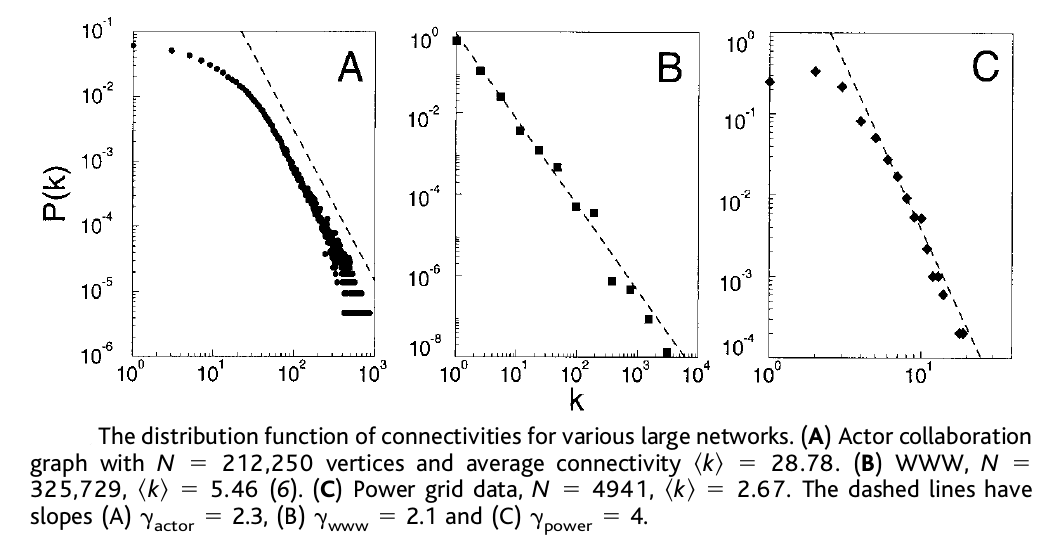
\includegraphics[scale=0.4]{../Images/BAResults.png}
\end{figure}


%---------------Start garbage----------------------%
~~insert wikipedia results here~~

Now that we know the odds of finding a knot in Wikipedia, we want to know if this probability is characteristic of solely Wikipedia, or if it’s a property of the types of graphs that Wikipedia resembles. So we tested what kind of graph Wikipedia was. We checked against four types of graphs:
1. Truly random graphs, created by the Erdos-Renyi algorithm
2. Semi-small world, highly connected graphs, generated by the Watts-Strogatz algorithm
3. Truly small world graphs, generated by the Barabasi-Albert algorithm
4. None of the above

Our hypothesis was that the subgraphs we analyzed were characteristically small world graphs. So we plotted the clustering coefficient of the graphs against the number of vertices. The result are in the figure below.

<insert clustering/vertex figure here />

The figure indicates that Wikipedia subgraphs cluster in a similar manner to truly small-world graphs. As a result, we generated a sample of Barabasi-Albert graphs similar in size to the 600 Wikipedia graphs we had, and checked the probability that these graphs had a knot. 

If the probability is similar, discuss implications
If the probability is not similar, discuss differences between BA and wikipedia
\section{Knots in other types of graphs}
\section{Conclusion}

\end{document}